\documentclass{article}%
\usepackage[T1]{fontenc}%
\usepackage[utf8]{inputenc}%
\usepackage{lmodern}%
\usepackage{textcomp}%
\usepackage{lastpage}%
\usepackage{authblk}%
\usepackage{graphicx}%
%
\title{Signaling pathway underlying the up{-}regulatory effect of TNF{-}a on the Na+/K+ ATPase in HepG2 cells}%
\author{Jeffrey Carroll MD}%
\affil{Department of Pediatrics and Molecular and Cellular Oncology, The University of Texas M. D. Anderson Cancer Center, Houston, TX, USA}%
\date{01{-}01{-}2012}%
%
\begin{document}%
\normalsize%
\maketitle%
\section{Abstract}%
\label{sec:Abstract}%
SAN DIEGO {-} The prebiological effect of caffeine on hepato\_ carcinogenesis {-} the characteristic lysine{-}like agents of the liver {-} and the protective effect of curcumin on chronic drug exposure appears to be well known. The latest research investigating the effects of these compounds in humans is being conducted at the Center for Investigational Antibiotic \& Drug Discovery (CIDD), at The Scripps Research Institute (TSRI).\newline%
Dr. Steven A. Nadel, Distinguished Professor in the Laboratory of Pharmacology and Toxicology and Director of the Center for Investigational Antibiotic \& Drug Discovery (CIDD), says, "This research, designed to elucidate the systemic pathways involved in hepato\_ carcinogenesis in humans, has the potential to have significant implications for prevention of liver cancer and drug resistance to existing therapies."\newline%
Tests of the percumin and curcumin compounds were performed on rats who had been genetically engineered to inherit extra copies of these beneficial proteins, adding a function associated with the human tropis cells. The result was that the parasites switched on and off their own beneficial quercetin compounds and fed directly onto the test tubes. The results showed that the quercetin compounds, which were found to enhance hepato\_ carcinogenesis in low doses by activating perchlorate receptors in the liver, were directly activated by the quercetin molecules in rats who became infected with hepatitis that originates in the central nervous system of animals and humans. They showed no genetic differences between the rats whose genetic material had been altered to be hepatitis{-}resistant, but were still susceptible to chronic Hepatitis B infection.\newline%
Dr. Nadel's laboratory at the Scripps Research Institute, where he directs the Rat Cancer Research Center, is regularly collaborating with the Scripps Research Institute (TSRI) to modify strains of mutated rat pupuscule {-} the tiny biological parts that code for proteins {-} that are presented in major viral pathogens such as Varicella zoster virus (Zoster) and cardiovasculitis.\newline%
"This is the first time that the problem of mutant rat pupuscule has been posed to a synthetic model to test its effectiveness," he says.\newline%
Nadel says that the promising results in rats show that the toxicity of these compounds should be evaluated in larger animals before large populations of rats are subjected to their toxicity in humans.\newline%
"The results of this study provide an important hint about how drugs might be modified in order to effect this beneficial effect on infected human subjects," he says. "Our next step is to establish the safety of these compounds against hepatotoxicity, virus toxicity and mutagenesis."

%
\subsection{Image Analysis}%
\label{subsec:ImageAnalysis}%


\begin{figure}[h!]%
\centering%
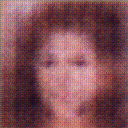
\includegraphics[width=150px]{500_fake_images/samples_5_276.png}%
\caption{A Man In A Suit And Tie Is Smiling}%
\end{figure}

%
\end{document}